\documentclass[UTF8,a4paper,10pt, twocolumn]{ctexart}
\usepackage[left=2.50cm, right=2.50cm, top=2.50cm, bottom=2.50cm]{geometry}

% -- text font --
% compile using Xelatex

%\setmainfont{Microsoft YaHei}  % 微软雅黑
%\setmainfont{YouYuan}  % 幼圆
%\setmainfont{NSimSun}  % 新宋体
%\setmainfont{KaiTi}    % 楷体
%\setmainfont{SimSun}   % 宋体
%\setmainfont{SimHei}   % 黑体

\usepackage{times}
%\usepackage{mathpazo}
%\usepackage{fourier}
%\usepackage{charter}
%\usepackage{helvet}

\usepackage{amsmath, amsfonts, amssymb} % math equations, symbols
\usepackage[english]{babel}
\usepackage{color}      % color content
\usepackage{graphicx}   % import figures
\usepackage{url}        % hyperlinks
\usepackage{bm}         % bold type for equations
\usepackage{multirow}
\usepackage{booktabs}
\usepackage{epstopdf}
\usepackage{epsfig}
\usepackage{algorithm}
\usepackage{algorithmic}
\renewcommand{\algorithmicrequire}{ \textbf{Input:}}     % use Input in the format of Algorithm
\renewcommand{\algorithmicensure}{ \textbf{Initialize:}} % use Initialize in the format of Algorithm
\renewcommand{\algorithmicreturn}{ \textbf{Output:}}     % use Output in the format of Algorithm

\usepackage{fancyhdr}   % 设置页眉、页脚
%\pagestyle{fancy}
\lhead{}
\chead{}
%\rhead{\includegraphics[width=1.2cm]{fig/ZJU_BLUE.eps}}
\lfoot{}
\cfoot{}
\rfoot{}

\usepackage{draftwatermark}         % 所有页加水印
%\usepackage[firstpage]{draftwatermark} % 只有第一页加水印
%\SetWatermarkText{Water-Mark}           % 设置水印内容
%\SetWatermarkText{\includegraphics{fig/ZJDX-WaterMark.eps}}         % 设置水印logo
%\SetWatermarkLightness{0.9}             % 设置水印透明度 0-1
%\SetWatermarkScale{1}                   % 设置水印大小 0-1

\usepackage{hyperref}   % bookmarks
\hypersetup{colorlinks, bookmarks, unicode} % unicode


\title{仿冒APP识别工具的设计与实现}
\author{ 程潇 2018111027  \thanks{组长}\\
垢宇晴 2018111037  \thanks{组员}\\
王皓 2018110990  \thanks{组员}
}

\date{\today}

\begin{document}
    \maketitle
    \thispagestyle{fancy}

\section{研究背景与意义} \label{sec:one}
    第\ref{sec:one}章的主要内容是研究的背景与意义。
\subsection{移动终端的飞速发展}
目前,移动设备的使用频率已经超过了PC端,并且移动设备中储存了更多没有备份过的个人信息、甚至企业数据,一旦泄露,后果将无法弥补

\subsection{仿冒App层出不穷}
App开发者由于缺少审核机制,恶意软件开发商可以轻易地发布一些仿冒的产品,因此山寨的应用层出不穷

\subsection{课题目标}
设计并实现一个检测假冒应用程序的工具

\section{关键技术和实践难点} \label{sec:two}
   第\ref{sec:two}章的主要内容是关键技术和实践难点。
\subsection{metadata数据对比——短文本相似度}
\subsubsection{提取数据}
选取$metadata$中的$description\_html$字段。

\subsubsection{文本预处理}
1. 去掉所有带符号的词,如邮箱后缀、$hyphen$连词、缩写等;

2. 去掉非英文的词汇;

3.小写化;

4.去长度小于3的单词,去掉数字和包含符号的单词;

5.去除'the'、'about'等停用词;

6.进行词性标记,标记每个词的词性;

7.进行词形还原,去掉单词的词缀,提取单词的主干部分;

8.计算各个$token$的$TFIDF$值,即"词频-逆文本频率"

\subsubsection{训练模型}
1.基于预处理的文本,建立词向量,采用$Skip-Gram$训练神经网络,优化收敛词向量;

2.将训练好的模型和文本序列化至本地。

\subsection{metadata其他数据对比}
\subsubsection{字符串相似度}
1.选取$metadata$中的$title$、$package\_name$、$developer\_email$等字段;

2.采用字符串的编辑距离度量相似度。

\subsubsection{特征向量相似度}
1.选取$metadata$中的$app\_category$、$app\_type$、$permission$等字段;

2.建立词汇表,取词汇表下标并进行归一化,将最后所得数值作为特征向量;

3.计算特征向量间的余弦相似度。

\subsection{$apk\_icon$对比——感知哈希算法}
对每张图片生成一个"指纹"(fingerprint)字符串,然后比较不同图片的指纹。结果越接近,就说明图片越相似。步骤如下:

1. 第一步,缩小尺寸。将图片缩小到8x8的尺寸,总共64个像素。这一步的作用是去除图片的细节,只保留结构、明暗等基本信息,摒弃不同尺寸、比例带来的图片差异。

2.第二步,简化色彩。将缩小后的图片,转为64级灰度。也就是说,所有像素点总共只有64种颜色。

3.第三步,计算平均值。计算所有64个像素的灰度平均值。

4. 第四步,比较像素的灰度。将每个像素的灰度,与平均值进行比较。大于或等于平均值,记为1;小于平均值,记为0。

5. 第五步,计算哈希值。将上一步的比较结果,组合在一起,就构成了一个64位的整数,这就是这张图片的指纹。组合的次序并不重要,只要保证所有图片都采用同样次序就行了。

得到指纹以后,就可以对比不同的图片,看看64位中有多少位是不一样的。理论上,这等同于计算汉明距离($Hamming distance$)。如果不相同的数据位不超过5,就说明两张图片很相似;如果大于10,就说明这是两张不同的图片。

\section{成果展示}
\subsection{metadata数据对比}
选取$metadata$中的$description\_html$字段,对比如图。

\begin{figure}[htbp]
\centering
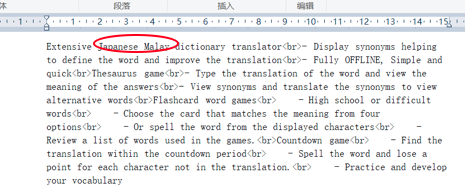
\includegraphics[width=0.2\textwidth]{img/fig1.png}
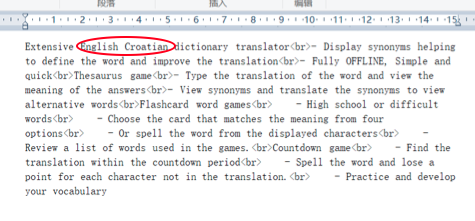
\includegraphics[width=0.2\textwidth]{img/fig2.png}
\caption{相似度为0.999999963的两段文本对比}
\label{figure:zju1}
\end{figure}

\begin{figure}[htbp]
  \centering
  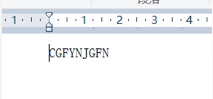
\includegraphics[width=0.2\textwidth]{img/fig3.png}
  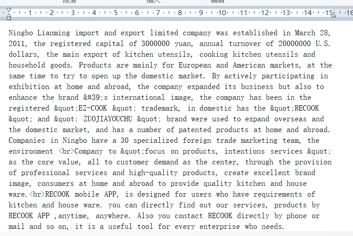
\includegraphics[width=0.2\textwidth]{img/fig4.png}
  \caption{相似度为0.173356448的两段文本对比}
  \label{figure:zju2}
  \end{figure}

\end{document}